%%%%%%%%%%%%%%%%%%%%%%%%%%%%%%%%%%%%%%%%%%%%%%%%%%%%%%%%%%%%%%%%%%%%%%%%%%%%
% AGUtmpl.tex: this template file is for articles formatted with LaTeX2e,
% Modified December 2018
%
% This template includes commands and instructions
% given in the order necessary to produce a final output that will
% satisfy AGU requirements.
%
% FOR FIGURES, DO NOT USE \psfrag
%
%%%%%%%%%%%%%%%%%%%%%%%%%%%%%%%%%%%%%%%%%%%%%%%%%%%%%%%%%%%%%%%%%%%%%%%%%%%%
%
% IMPORTANT NOTE:
%
% SUPPORTING INFORMATION DOCUMENTATION IS NOT COPYEDITED BEFORE PUBLICATION.
%
%
%
%%%%%%%%%%%%%%%%%%%%%%%%%%%%%%%%%%%%%%%%%%%%%%%%%%%%%%%%%%%%%%%%%%%%%%%%%%%%
%
% Step 1: Set the \documentclass
%
%
% PLEASE USE THE DRAFT OPTION TO SUBMIT YOUR PAPERS.
% The draft option produces double spaced output.
%
% Choose the journal abbreviation for the journal you are
% submitting to:

% jgrga JOURNAL OF GEOPHYSICAL RESEARCH (use for all of them)
% gbc   GLOBAL BIOCHEMICAL CYCLES
% grl   GEOPHYSICAL RESEARCH LETTERS
% pal   PALEOCEANOGRAPHY
% ras   RADIO SCIENCE
% rog   REVIEWS OF GEOPHYSICS
% tec   TECTONICS
% wrr   WATER RESOURCES RESEARCH
% gc    GEOCHEMISTRY, GEOPHYSICS, GEOSYSTEMS
% sw    SPACE WEATHER
% ms    JAMES
% ef    EARTH'S FUTURE
%
%
%
% (If you are submitting to a journal other than jgrga,
% substitute the initials of the journal for "jgrga" below.)

\documentclass[draft,ms]{agutexSI2019}
\usepackage{longtable}
\usepackage{amsmath}
\usepackage{amssymb}
\usepackage{bm}
\usepackage{graphicx}
\usepackage{epstopdf}
\usepackage{xcolor}
\usepackage{hyperref}
\DeclareGraphicsRule{.tif}{png}{.png}{`convert #1 `basename #1 .tif`.png}
\usepackage{color}
\usepackage{longtable}
\usepackage{textcomp}
\graphicspath{{../../../etc/plots/climate_et/test_plots/}}
\newcommand\newblock{\hskip .11em\@plus.33em\@minus.07em}

\RequirePackage{natbib}

%%%%%%%%%%%%%%%%%%%%%%%%%%%%%%%%%%%%%%%%%%%%%%%%%%%%%%%%%%%%%%%%%%%%%%%%%
%
%  SUPPORTING INFORMATION TEMPLATE
%
%% ------------------------------------------------------------------------ %%
%
%
%Please use this template when formatting and submitting your Supporting Information.

%This template serves as both a “table of contents” for the supporting information for your article and as a summary of files.
%
%
%OVERVIEW
%
%Please note that all supporting information will be peer reviewed with your manuscript. It will not be copyedited if the paper is accepted.
%In general, the purpose of the supporting information is to enable authors to provide and archive auxiliary information such as data tables, method information, figures, video, or computer software, in digital formats so that other scientists can use it.
%The key criteria are that the data:
% 1. supplement the main scientific conclusions of the paper but are not essential to the conclusions (with the exception of
%    including %data so the experiment can be reproducible);
% 2. are likely to be usable or used by other scientists working in the field;
% 3. are described with sufficient precision that other scientists can understand them, and
% 4. are not exe files.
%
%USING THIS TEMPLATE
%
%***All references should be included in the reference list of the main paper so that they can be indexed, linked, and counted as citations.  The reference section does not count toward length limits.
%
%All Supporting text and figures should be included in this document. Insert supporting information content into each appropriate section of the template. To add additional captions, simply copy and paste each sample as needed.

%Tables may be included, but can also be uploaded separately, especially if they are larger than 1 page, or if necessary for retaining table formatting. Data sets, large tables, movie files, and audio files should be uploaded separately. Include their captions in this document and list the file name with the caption. You will be prompted to upload these files on the Upload Files tab during the submission process, using file type “Supporting Information (SI)”

%IMPORTANT NOTE ON FIGURES AND TABLES
% Placeholders for figures and tables appear after the \end{article} command, after references.
% DO NOT USE \psfrag or \subfigure commands.
%
 \usepackage{graphicx}
%
%  Uncomment the following command to allow illustrations to print
%   when using Draft:
 \setkeys{Gin}{draft=false}
%
% You may need to use one of these options for graphicx depending on the driver program you are using.
%
% [xdvi], [dvipdf], [dvipsone], [dviwindo], [emtex], [dviwin],
% [pctexps],  [pctexwin],  [pctexhp],  [pctex32], [truetex], [tcidvi],
% [oztex], [textures]
%
%
%% ------------------------------------------------------------------------ %%
%
%  ENTER PREAMBLE
%
%% ------------------------------------------------------------------------ %%

% Author names in capital letters:
%\authorrunninghead{BALES ET AL.}

% Shorter version of title entered in capital letters:
%\titlerunninghead{SHORT TITLE}

%Corresponding author mailing address and e-mail address:
%\authoraddr{Corresponding author: A. B. Smith,
%Department of Hydrology and Water Resources, University of
%Arizona, Harshbarger Building 11, Tucson, AZ 85721, USA.
%(a.b.smith@hwr.arizona.edu)}

\begin{document}

%% ------------------------------------------------------------------------ %%
%
%  TITLE
%
%% ------------------------------------------------------------------------ %%

%\includegraphics{agu_pubart-white_reduced.eps}


\title{Supporting Information for "When does vapor pressure deficit drive or reduce
  evapotranspiration?"}
%
% e.g., \title{Supporting Information for "Terrestrial ring current:
% Origin, formation, and decay $\alpha\beta\Gamma\Delta$"}
%
%DOI: 10.1002/%insert paper number here%

%% ------------------------------------------------------------------------ %%
%
%  AUTHORS AND AFFILIATIONS
%
%% ------------------------------------------------------------------------ %%


% List authors by first name or initial followed by last name and
% separated by commas. Use \affil{} to number affiliations, and
% \thanks{} for author notes.
% Additional author notes should be indicated with \thanks{} (for
% example, for current addresses).

% Example: \authors{A. B. Author\affil{1}\thanks{Current address, Antartica}, B. C. Author\affil{2,3}, and D. E.
% Author\affil{3,4}\thanks{Also funded by Monsanto.}}


\authors{A. Massmann\affil{1}, P. Gentine\affil{1}, C. Lin\affil{1,2}}


\affiliation{1}{Department of Earth and Environmental Engineering,
  Columbia University, New York, NY 10027}
\affiliation{2}{State Key Laboratory of Hydroscience and Engineering, Department of Hydraulic
  Engineering, Tsinghua University, Beijing, CN 100084}





%% ------------------------------------------------------------------------ %%
%
%  BEGIN ARTICLE
%
%% ------------------------------------------------------------------------ %%

% The body of the article must start with a \begin{article} command
%
% \end{article} must follow the references section, before the figures
%  and tables.

\begin{article}

%% ------------------------------------------------------------------------ %%
%
%  TEXT
%
%% ------------------------------------------------------------------------ %%



\noindent\textbf{Contents of this file}
%%%Remove or add items as needed%%%
\begin{enumerate}
\item Figures S1 to S68
\item Table S1
\end{enumerate}

\noindent\textbf{Introduction}

The manuscript analyzes the partial derivative of ET with respect to
VPD. This assumes that all other quantities remain fixed, including the
plant parameters g$_1$ and uWUE (and by extension, $\lambda$). In
reality, these parameters may vary with environmental conditions, and
specifically soil moisture. However because soil moisture
\textit{only} enters the partial derivative directly through these
plant terms, if the plant parameters are weak functions of soil
moisture then the theory can be directly applied to a broader range of
conceptual VPD scenarios, including observed compound events between
high VPD and low soil moisture \cite{Zhou_2019}. To help the reader
assess the soil moisture dependence of uWUE (and partially by
extension $\lambda$ and g$_1$), we provide here figures showing the
distribution of uWUE with SWC for each of 66 FLUXNET sites from the
FLUXNET-2015 database. The functional relationship between uWUE and
SWC varies, with a mix of sites showing strong and weak
SWC-dependence. For all sites the ratio of signal to noise is very
low, an unfortunate consequence of taking a ratio of two highly
uncertain eddy-covariance derived fluxes. In general we find this
analysis inconclusive.

The paper does not rely on assumptions about uWUE's functional
relationship with soil moisture so we do not include the figures in
the body of the manuscript. But given that constant uWUE and g$_1$
assumptions can make our theory more useful to the reader we provide
the figures for their interpretation, and motivation for future
research.

Additionally, we include a figure showing the joint distribution
between saturation vapor pressure and relative humidity calculated
from the FLUXNET-2015 data. Relative humidity and saturation vapor
pressure are much more independent than saturation vapor pressure and
VPD, and we use an assumption that relative humidity and saturation
vapor pressure can be approximated as independent in order to evaluate
$\frac{\partial ET}{\partial VPD}$. Please note that at a given site,
the relationship may be more or less independent depending on the
hydroclimate.


\section{Description of data}
\subsection{Data}
We use both meteorological and eddy-covariance data from the
FLUXNET2015 database (data available at \sloppy
\url{https://fluxnet.fluxdata.org/data/fluxnet2015-dataset/} \sloppy),
including all Tier 1 sites with at least four years of data. Sixty-six
sites met these requirements, and were grouped into nine plant
functional types (PFT) according to the International
Geosphere-Biosphere Programme vegetation classification scheme
\cite{Loveland_1999}: cropland (CRO), grass (GRA), deciduous
broadleaf forest (DBF), evergreen broadleaf forest (EBF), evergreen
needleleaf forest (ENF), mixed forest (MF), closed shrub (CSH),
savannah (SAV), and woody savannah (WSA).

\begin{figure}[h]
  \centering 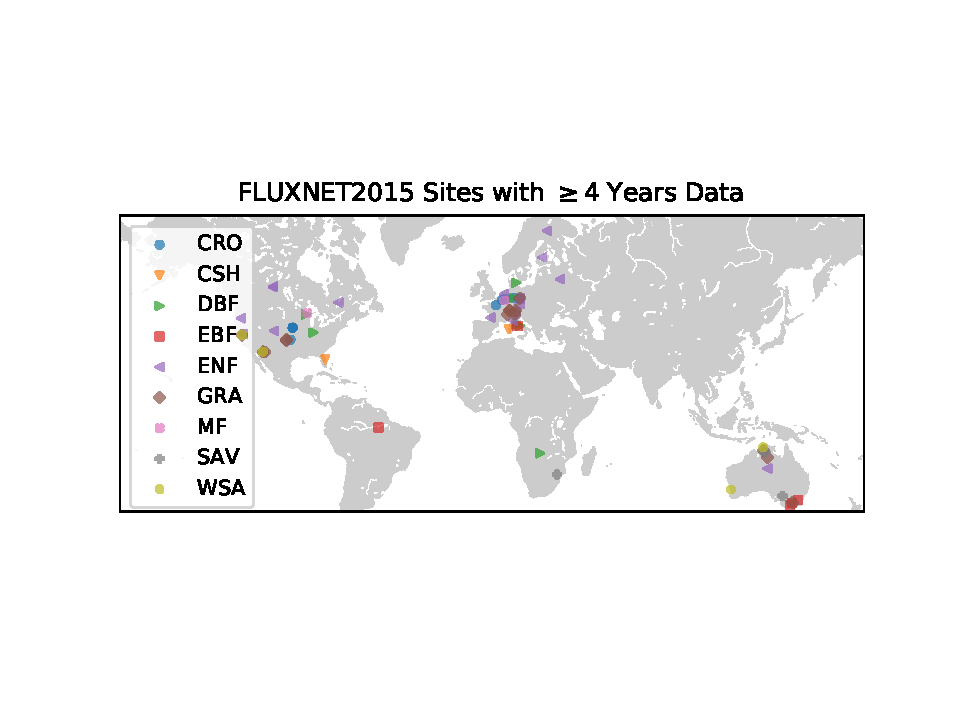
\includegraphics[trim={0 3cm 0 3cm}, clip]{./map.pdf}
  \caption{Plant functional type and location of FLUXNET2015 sites
    used in this analysis.}
  \label{map_fig}
\end{figure}
We filter and quality control the FLUXNET-2015 data using a similar
procedure as \cite{Zhou_2015}:

\begin{itemize}
\item Only measured or highest (``good'') quality gapfilled data,
  according to quality control flags, are used.
\item To isolate the growing season, we only use days in which the
  average Gross Primary Productivity (GPP) exceeds 10\% of the
  observed 95th percentile of GPP for a given site. GPP is calculated
  using the nighttime respiration partitioning method.
\item We remove days with rain and the day following to avoid issues
  with rain interception and sensor saturation at high relative
  humidity (\cite{Medlyn_2017}).
\item For SWC measurements, we use the shallowest observed layer
  available at each site.
\end{itemize}

Additionally, as in \citet{Lin_2018}, we restrict data to the daytime,
which is identified when downwelling shortwave radiation is greater
than 50 W m$^{-2}$ and sensible heat flux is greater than 5 W
m$^{-2}$. To reduce the chance of sensor saturation at high relative
humidity, we remove all time steps for which VPD is less than .01 kPa,
and to reduce errors at low windspeeds we remove all periods with wind
magnitudes less than 0.5 m s$^{-1}$. Timesteps with negative observed
GPP or ET are also removed, and we aggregate half hourly data to
hourly averages to reduce noise \cite{Lin_2018}.  After these quality
control procedures, 400,983 upscaled hourly observations remain.




\bibliography{references}

%\clearpage

%Delete all unused file types below. Copy/paste for multiples of each file type as needed.


%Repeat for any additional Supporting audio files

%%% End of body of article:
%%%%%%%%%%%%%%%%%%%%%%%%%%%%%%%%%%%%%%%%%%%%%%%%%%%%%%%%%%%%%%%%
%
% Optional Notation section goes here
%
% Notation -- End each entry with a period.
% \begin{notation}
% Term & definition.\\
% Second term & second definition.\\
% \end{notation}
%%%%%%%%%%%%%%%%%%%%%%%%%%%%%%%%%%%%%%%%%%%%%%%%%%%%%%%%%%%%%%%%


%% ------------------------------------------------------------------------ %%
%%  REFERENCE LIST AND TEXT CITATIONS

%%%%%%%%%%%%%%%%%%%%%%%%%%%%%%%%%%%%%%%%%%%%%%%
%
%
% \bibliography{<name of your .bib file>} do not specify file extension
%
% no need to specify bibliographystyle
%
% Note that ALL references in this supporting information file must also be referenced in the primary manuscript
%
%%%%%%%%%%%%%%%%%%%%%%%%%%%%%%%%%%%%%%%%%%%%%%%
% if you get an error about newblock being undefined, uncomment this line:
%\newcommand{\newblock}{}

% \bibliography{ uncomment this line and enter the name of your bibtex file here }




%Reference citation instructions and examples:
%
% Please use ONLY \cite and \citeA for reference citations.
% \cite for parenthetical references
% ...as shown in recent studies (Simpson et al., 2019)
% \citeA for in-text citations
% ...Simpson et al (2019) have shown...
% DO NOT use other cite commands (e.g., \citet, \citep, \citeyear, \nocite, \citealp, etc.).
%
%
%...as shown by \citeA{jskilby}.
%...as shown by \citeA{lewin76}, \citeA{carson86}, \citeA{bartoldy02}, and \citeA{rinaldi03}.
%...has been shown \cite<e.g.,>{jskilbye}.
%...has been shown \cite{lewin76,carson86,bartoldy02,rinaldi03}.
%...has been shown \cite{lewin76,carson86,bartoldy02,rinaldi03}.
%
% apacite uses < > for prenotes, not [ ]
% DO NOT use other cite commands (e.g., \citet, \citep, \citeyear, \nocite, \citealp, etc.).
%

%% ------------------------------------------------------------------------ %%
%
%  END ARTICLE
%
%% ------------------------------------------------------------------------ %%
\end{article}
\clearpage

% Copy/paste for multiples of each file type as needed.

% enter figures and tables below here: %%%%%%%


\begin{figure}
  \centering \includegraphics{./supp-figs/0joint_rh_es.pdf}
  \caption{The joint distribution of relative humidity and saturation
    vapor pressure for the FLUXNET2015 dataset.}
  \end{figure}

\input{supp-figs.tex}


% tables


  % below taken adapted from Trevor Keenan's FLUXNET citations
  % at github.com/trevorkeenan/FLUXNET_citations
  Table S1: Metadata and citations for flux sites used in this analysis. All data are gathered from \url{www.fluxdata.org}, and citations are aggregated using tools available at \url{https://github.com/trevorkeenan/FLUXNET_citations}.
  \begin{longtable}{l l l l l l l}
    \hline
    \textbf{Site} &
    \textbf{PFT} &
    \textbf{Lat} &
    \textbf{Lon} &
    \textbf{Clim\textsuperscript{1}} &
    \textbf{Period} &
    \textbf{References} \\
    [0.5ex]
    \hline
    AT-Neu & GRA & 47.1167 & 11.3175 & Unk & 2002-2012 & \cite{AT-Neu} \\
AU-ASM & ENF & -22.2830 & 133.2490 & Unk & 2010-2013 & \cite{AU-ASM} \\
AU-Cpr & SAV & -34.0021 & 140.5891 & Unk & 2010-2014 & \cite{AU-Cpr} \\
AU-DaP & GRA & -14.0633 & 131.3181 & Aw  & 2007-2013 & \cite{AU-DaP} \\
AU-DaS & SAV & -14.1593 & 131.3881 & Aw  & 2008-2014 & \cite{AU-DaS} \\
AU-Dry & SAV & -15.2588 & 132.3706 & Unk & 2008-2014 & \cite{AU-Dry} \\
AU-Gin & WSA & -31.3764 & 115.7138 & Unk & 2011-2014 & \cite{AU-Gin} \\
AU-How & WSA & -12.4943 & 131.1523 & Aw  & 2001-2014 & \cite{AU-How} \\
AU-Rig & GRA & -36.6499 & 145.5759 & Unk & 2011-2014 & \cite{AU-Gin} \\
AU-Stp & GRA & -17.1507 & 133.3502 & Unk & 2008-2014 & \cite{AU-DaP} \\
AU-Tum & EBF & -35.6566 & 148.1517 & Cfb & 2001-2014 & \cite{AU-Tum} \\
AU-Whr & EBF & -36.6732 & 145.0294 & Unk & 2011-2014 & \cite{AU-Whr} \\
AU-Wom & EBF & -37.4222 & 144.0944 & Unk & 2010-2012 & \cite{AU-Wom} \\
BE-Lon & CRO & 50.5516 & 4.7461 & Cfb & 2004-2014 & \cite{BE-Lon} \\
BE-Vie & MF & 50.3051 & 5.9981 & Cfb & 1996-2014 & \cite{BE-Vie} \\
BR-Sa3 & EBF & -3.0180 & -54.9714 & Am & 2000-2004 & \cite{BR-Sa3} \\
CA-Qfo & ENF & 49.6925 & -74.3421 & Dfc & 2003-2010 & \cite{CA-Qfo} \\
CA-SF1 & ENF & 54.4850 & -105.8176 & Dfc & 2003-2006 & \cite{CA-SF1} \\
CA-SF2 & ENF & 54.2539 & -105.8775 & Dfc & 2001-2005 & \cite{CA-SF1} \\
CH-Cha & GRA & 47.2102 & 8.4104 & Unk & 2005-2014 & \cite{CH-Cha} \\
CH-Dav & ENF & 46.8153 & 9.8559 & Unk & 1997-2014 & \cite{CH-Dav} \\
CH-Fru & GRA & 47.1158 & 8.5378 & Unk & 2005-2014 & \cite{CH-Fru} \\
DE-Geb & CRO & 51.1001 & 10.9143 & Unk & 2001-2014 & \cite{DE-Geb} \\
DE-Gri & GRA & 50.9500 & 13.5126 & Cfb & 2004-2014 & \cite{DE-Gri} \\
DE-Hai & DBF & 51.0792 & 10.4530 & Unk & 2000-2012 & \cite{DE-Hai} \\
DE-Kli & CRO & 50.8931 & 13.5224 & Cfb & 2004-2014 & \cite{DE-Gri} \\
DE-Lkb & ENF & 49.0996 & 13.3047 & Unk & 2009-2013 & \cite{DE-Lkb} \\
DE-Obe & ENF & 50.7867 & 13.7213 & Cfb & 2008-2014 & {\textendash} \\
DE-Seh & CRO & 50.8706 & 6.4497 & Unk & 2007-2010 & \cite{DE-Seh} \\
DE-Tha & ENF & 50.9624 & 13.5652 & Cfb & 1996-2014 & \cite{DE-Tha} \\
DK-Sor & DBF & 55.4859 & 11.6446 & Unk & 1996-2014 & \cite{DK-Sor} \\
FI-Hyy & ENF & 61.8474 & 24.2948 & Unk & 1996-2014 & \cite{FI-Hyy} \\
FI-Sod & ENF & 67.3619 & 26.6378 & Unk & 2001-2014 & \cite{FI-Sod} \\
FR-Gri & CRO & 48.8442 & 1.9519 & Cfb & 2004-2013 & \cite{FR-Gri} \\
FR-LBr & ENF & 44.7171 & -0.7693 & Unk & 1996-2008 & \cite{FR-LBr} \\
IT-Col & DBF & 41.8494 & 13.5881 & Unk & 1996-2014 & \cite{IT-Col} \\
IT-Cpz & EBF & 41.7052 & 12.3761 & Unk & 1997-2009 & \cite{IT-Cpz} \\
IT-Lav & ENF & 45.9562 & 11.2813 & Unk & 2003-2014 & \cite{IT-Lav} \\
IT-MBo & GRA & 46.0147 & 11.0458 & Unk & 2003-2013 & \cite{IT-MBo} \\
IT-Noe & CSH & 40.6061 & 8.1515 & Unk & 2004-2014 & \cite{IT-Noe} \\
IT-Ren & ENF & 46.5869 & 11.4337 & Unk & 1998-2013 & \cite{IT-Ren} \\
IT-Ro2 & DBF & 42.3903 & 11.9209 & Unk & 2002-2012 & \cite{IT-Ro2} \\
IT-SRo & ENF & 43.7279 & 10.2844 & Unk & 1999-2012 & \cite{IT-SRo} \\
IT-Tor & GRA & 45.8444 & 7.5781 & Unk & 2008-2014 & \cite{IT-Tor} \\
NL-Loo & ENF & 52.1666 & 5.7436 & Unk & 1996-2013 & \cite{NL-Loo} \\
RU-Fyo & ENF & 56.4615 & 32.9221 & Unk & 1998-2014 & \cite{RU-Fyo} \\
US-AR1 & GRA & 36.4267 & -99.4200 & Dsa & 2009-2012 & \cite{US-AR1} \\
US-AR2 & GRA & 36.6358 & -99.5975 & Dsa & 2009-2012 & \cite{US-AR1} \\
US-ARM & CRO & 36.6058 & -97.4888 & Cfa & 2003-2012 & \cite{US-ARM} \\
US-Blo & ENF & 38.8953 & -120.6328 & Csa & 1997-2007 & \cite{US-Blo} \\
US-KS2 & CSH & 28.6086 & -80.6715 & Cwa & 2003-2006 & \cite{US-KS2} \\
US-MMS & DBF & 39.3232 & -86.4131 & Cfa & 1999-2014 & \cite{US-MMS} \\
US-Me2 & ENF & 44.4523 & -121.5574 & Csb & 2002-2014 & \cite{US-Me2} \\
US-NR1 & ENF & 40.0329 & -105.5464 & Dfc & 1998-2014 & \cite{US-NR1} \\
US-Ne1 & CRO & 41.1651 & -96.4766 & Dfa & 2001-2013 & \cite{US-Ne1} \\
US-Ne2 & CRO & 41.1649 & -96.4701 & Dfa & 2001-2013 & \cite{US-Ne1} \\
US-Ne3 & CRO & 41.1797 & -96.4397 & Dfa & 2001-2013 & \cite{US-Ne1} \\
US-SRG & GRA & 31.7894 & -110.8277 & Bsk & 2008-2014 & \cite{US-SRG} \\
US-SRM & WSA & 31.8214 & -110.8661 & Bsk & 2004-2014 & \cite{US-SRM} \\
US-Syv & MF & 46.2420 & -89.3477 & Dfb & 2001-2014 & \cite{US-Syv} \\
US-Ton & WSA & 38.4316 & -120.9660 & Csa & 2001-2014 & \cite{US-Ton} \\
US-Var & GRA & 38.4133 & -120.9507 & Csa & 2000-2014 & \cite{US-Var} \\
US-WCr & DBF & 45.8059 & -90.0799 & Dfb & 1999-2014 & \cite{US-WCr} \\
US-Wkg & GRA & 31.7365 & -109.9419 & Bsk & 2004-2014 & \cite{US-Wkg} \\
ZA-Kru & SAV & -25.0197 & 31.4969 & Unk & 2000-2010 & \cite{ZA-Kru} \\
ZM-Mon & DBF & -15.4378 & 23.2528 & Unk & 2000-2009 & \cite{ZM-Mon} \\

    [1ex]
    \hline
  \end{longtable}
\textsuperscript{1} K{\"o}ppen Climate classification.


\end{document}

%%%%%%%%%%%%%%%%%%%%%%%%%%%%%%%%%%%%%%%%%%%%%%%%%%%%%%%%%%%%%%%

More Information and Advice:

%% ------------------------------------------------------------------------ %%
%
%  SECTION HEADS
%
%% ------------------------------------------------------------------------ %%

% Capitalize the first letter of each word (except for
% prepositions, conjunctions, and articles that are
% three or fewer letters).

% AGU follows standard outline style; therefore, there cannot be a section 1 without
% a section 2, or a section 2.3.1 without a section 2.3.2.
% Please make sure your section numbers are balanced.
% ---------------
% Level 1 head
%
% Use the \section{} command to identify level 1 heads;
% type the appropriate head wording between the curly
% brackets, as shown below.
%
%An example:
%\section{Level 1 Head: Introduction}
%
% ---------------
% Level 2 head
%
% Use the \subsection{} command to identify level 2 heads.
%An example:
%\subsection{Level 2 Head}
%
% ---------------
% Level 3 head
%
% Use the \subsubsection{} command to identify level 3 heads
%An example:
%\subsubsection{Level 3 Head}
%
%---------------
% Level 4 head
%
% Use the \subsubsubsection{} command to identify level 3 heads
% An example:
%\subsubsubsection{Level 4 Head} An example.
%
%% ------------------------------------------------------------------------ %%
%
%  IN-TEXT LISTS
%
%% ------------------------------------------------------------------------ %%
%
% Do not use bulleted lists; enumerated lists are okay.
% \begin{enumerate}
% \item
% \item
% \item
% \end{enumerate}
%
%% ------------------------------------------------------------------------ %%
%
%  EQUATIONS
%
%% ------------------------------------------------------------------------ %%

% Single-line equations are centered.
% Equation arrays will appear left-aligned.

Math coded inside display math mode \[ ...\]
 will not be numbered, e.g.,:
 \[ x^2=y^2 + z^2\]

 Math coded inside \begin{equation} and \end{equation} will
 be automatically numbered, e.g.,:
 \begin{equation}
 x^2=y^2 + z^2
 \end{equation}

% IF YOU HAVE MULTI-LINE EQUATIONS, PLEASE
% BREAK THE EQUATIONS INTO TWO OR MORE LINES
% OF SINGLE COLUMN WIDTH (20 pc, 8.3 cm)
% using double backslashes (\\).

% To create multiline equations, use the
% \begin{eqnarray} and \end{eqnarray} environment
% as demonstrated below.
\begin{eqnarray}
  x_{1} & = & (x - x_{0}) \cos \Theta \nonumber \\
        && + (y - y_{0}) \sin \Theta  \nonumber \\
  y_{1} & = & -(x - x_{0}) \sin \Theta \nonumber \\
        && + (y - y_{0}) \cos \Theta.
\end{eqnarray}

%If you don't want an equation number, use the star form:
%\begin{eqnarray*}...\end{eqnarray*}

% Break each line at a sign of operation
% (+, -, etc.) if possible, with the sign of operation
% on the new line.

% Indent second and subsequent lines to align with
% the first character following the equal sign on the
% first line.

% Use an \hspace{} command to insert horizontal space
% into your equation if necessary. Place an appropriate
% unit of measure between the curly braces, e.g.
% \hspace{1in}; you may have to experiment to achieve
% the correct amount of space.


%% ------------------------------------------------------------------------ %%
%
%  EQUATION NUMBERING: COUNTER
%
%% ------------------------------------------------------------------------ %%

% You may change equation numbering by resetting
% the equation counter or by explicitly numbering
% an equation.

% To explicitly number an equation, type \eqnum{}
% (with the desired number between the brackets)
% after the \begin{equation} or \begin{eqnarray}
% command.  The \eqnum{} command will affect only
% the equation it appears with; LaTeX will number
% any equations appearing later in the manuscript
% according to the equation counter.
%

% If you have a multiline equation that needs only
% one equation number, use a \nonumber command in
% front of the double backslashes (\\) as shown in
% the multiline equation above.

%% ------------------------------------------------------------------------ %%
%
%  SIDEWAYS FIGURE AND TABLE EXAMPLES
%
%% ------------------------------------------------------------------------ %%
%
% For tables and figures, add \usepackage{rotating} to the paper and add the rotating.sty file to the folder.
% AGU prefers the use of {sidewaystable} over {landscapetable} as it causes fewer problems.
%
% \begin{sidewaysfigure}
% \includegraphics[width=20pc]{samplefigure.eps}
% \caption{caption here}
% \label{label_here}
% \end{sidewaysfigure}
%
%
%
% \begin{sidewaystable}
% \caption{}
% \begin{tabular}
% Table layout here.
% \end{tabular}
% \end{sidewaystable}
%
%
